\chapter{Methods}
\section {Study Participants}
We measured 8 normal hearing people. Participant 8 was given silent stimuli as a comparison. The detailed information about the subjects are listed in the table.

\begin{table}[h!]
  \begin{center}
    
    
    \begin{tabular}{p{2.3cm} | p{1.5cm} |p{3cm} | p{3cm} | p{2.5cm} | p{1cm}} % <-- Alignments: 1st column left, 2nd middle and 3rd right, with vertical lines in between
      \textbf{Participant} & \textbf {Gender}& \textbf{Handedness} & \textbf{Race} & \textbf{Hair color} &\textbf {Age}\\ 
      \hline
      1 chang  & F & right-handed & east asian & dark & 22 yr \\
      2 gleb    & M & right-handed  & caucasian & blond & 18 \\
      3 jonas  & M & left-handed &  caucasian & brunet & 21\\
      4 lin      & F  & right-handed & east asian & dark& 21 \\
      5 lukas & M & right-handed  &  caucasian& blond & 26 \\
      6 shelia&  F & right-handed & southeast asian & dark & 22 \\
      7 liao.   &  M & right-handed &  east asian & dark & 22 \\
      8 lukas & M & right-handed  & caucasian & blond & 22 \\
    \end{tabular}
    \label{tab:table1}
    \caption{Study Participants.}
  \end{center}
  
\end{table}

\section {Probe Design}
The probes were first designed in AtlasViewer [pic] \cite {10.1117/1.NPh.2.2.020801} and the SD GUI interface. I tried to replicate the probe design as close as possible to the research from Weder et al. However, several modifications need to be made due to device limitations.

First of all, the paper only provided a rough 2D-sketch of their probe design. [see pic] The channels were not described in detail. Though there are different ways to define the channels, we believe it shouldn't matter as long as the mid-points of the channel correspond to that of the previous research.

\begin{figure}[H]
  \centering
    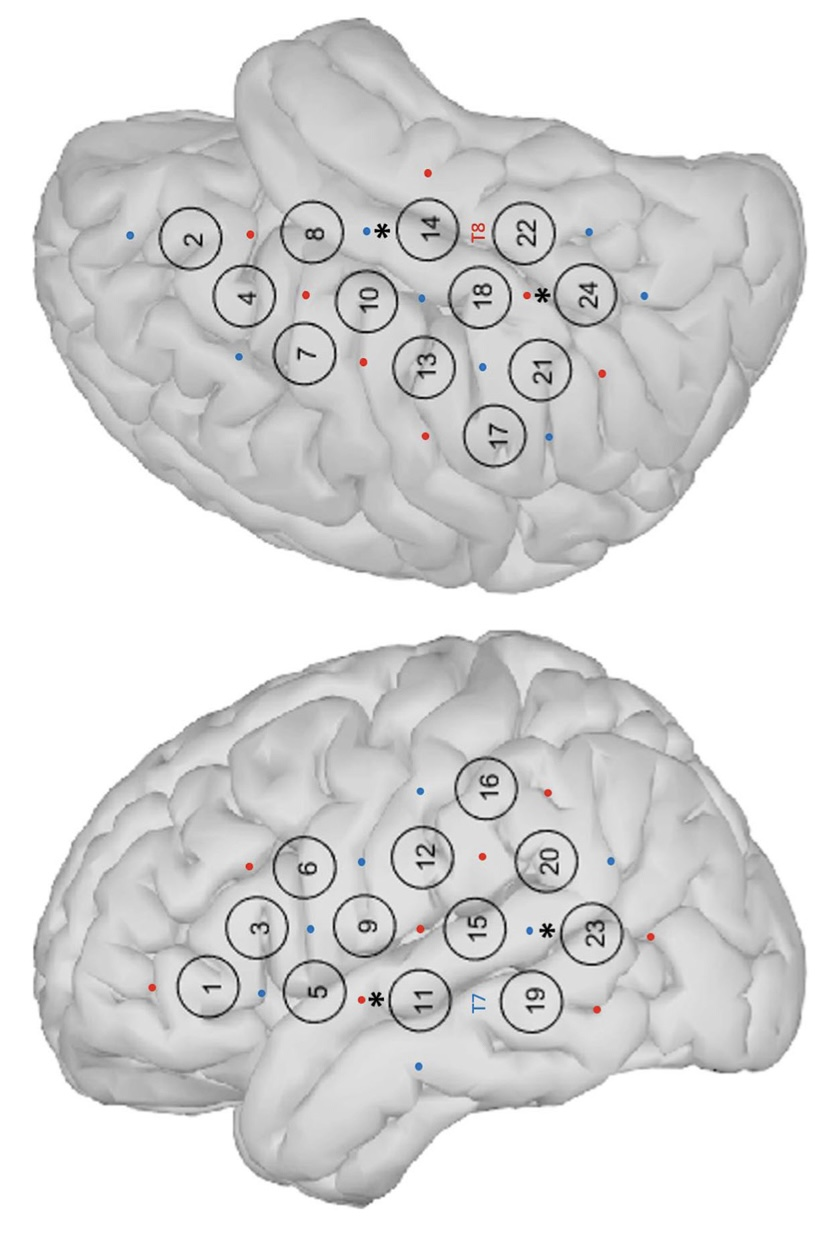
\includegraphics[scale= 0.4]{bilder/weder_probe.jpg}
  \caption{Probe design from Weder et al.}
  \label{fig:somesignal}
\end{figure}

\begin{figure}[H]
  \centering
    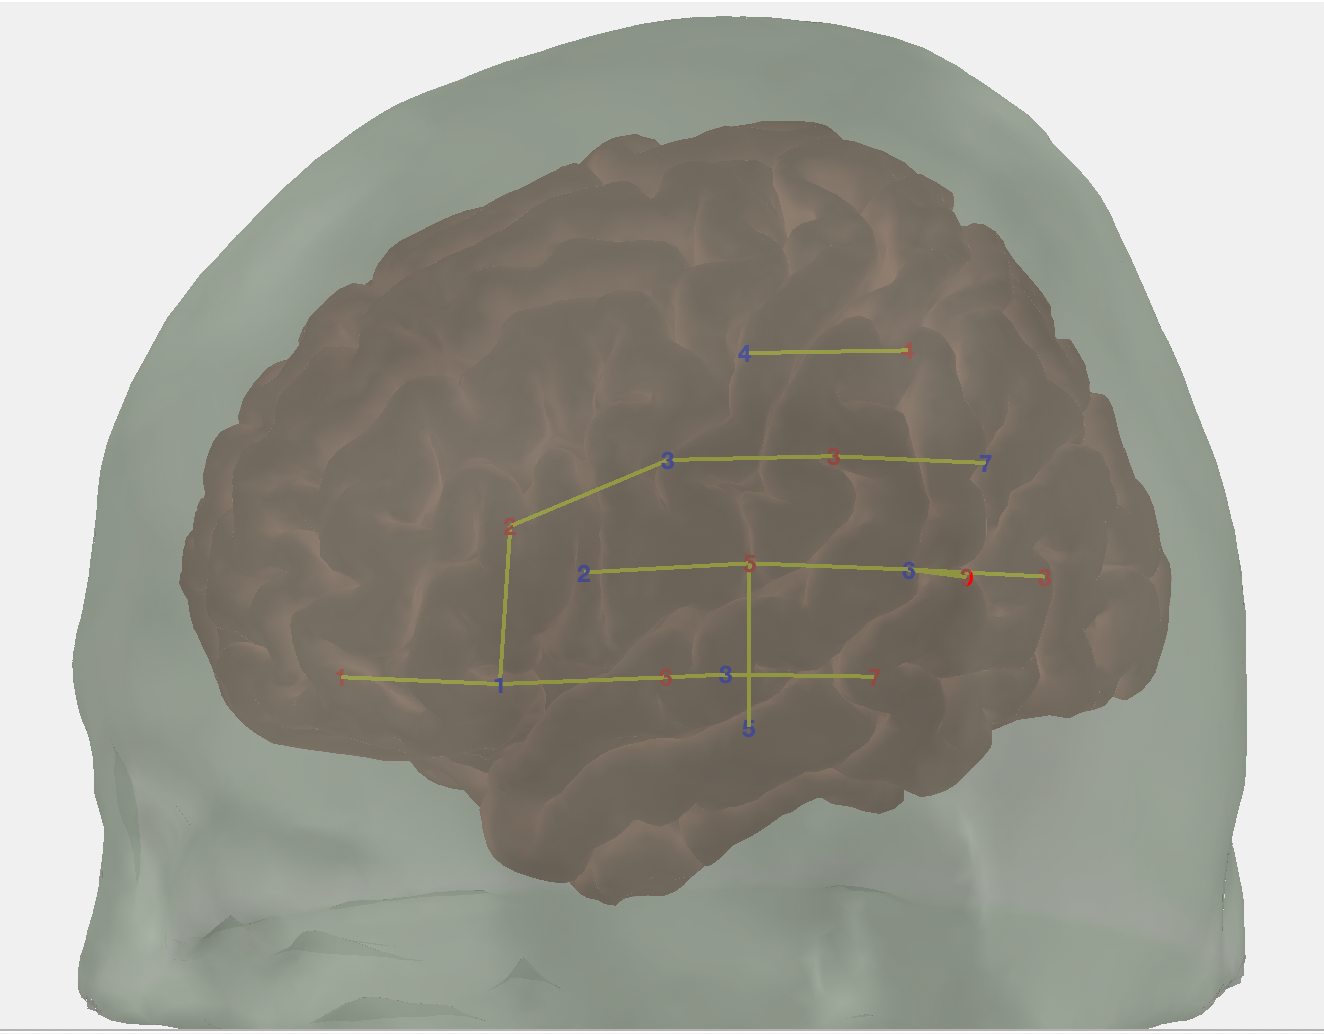
\includegraphics[scale=.35]{bilder/atlas_probe.png}
  \caption{Probe design in this research. Shown in AtlasViewer. The red numbers represent the light sources and the blue numbers represent the dectector. Channels are shown in yellow lines.}
  \label{fig:somesignal}
\end{figure}

\begin{figure}[H]
  \centering
    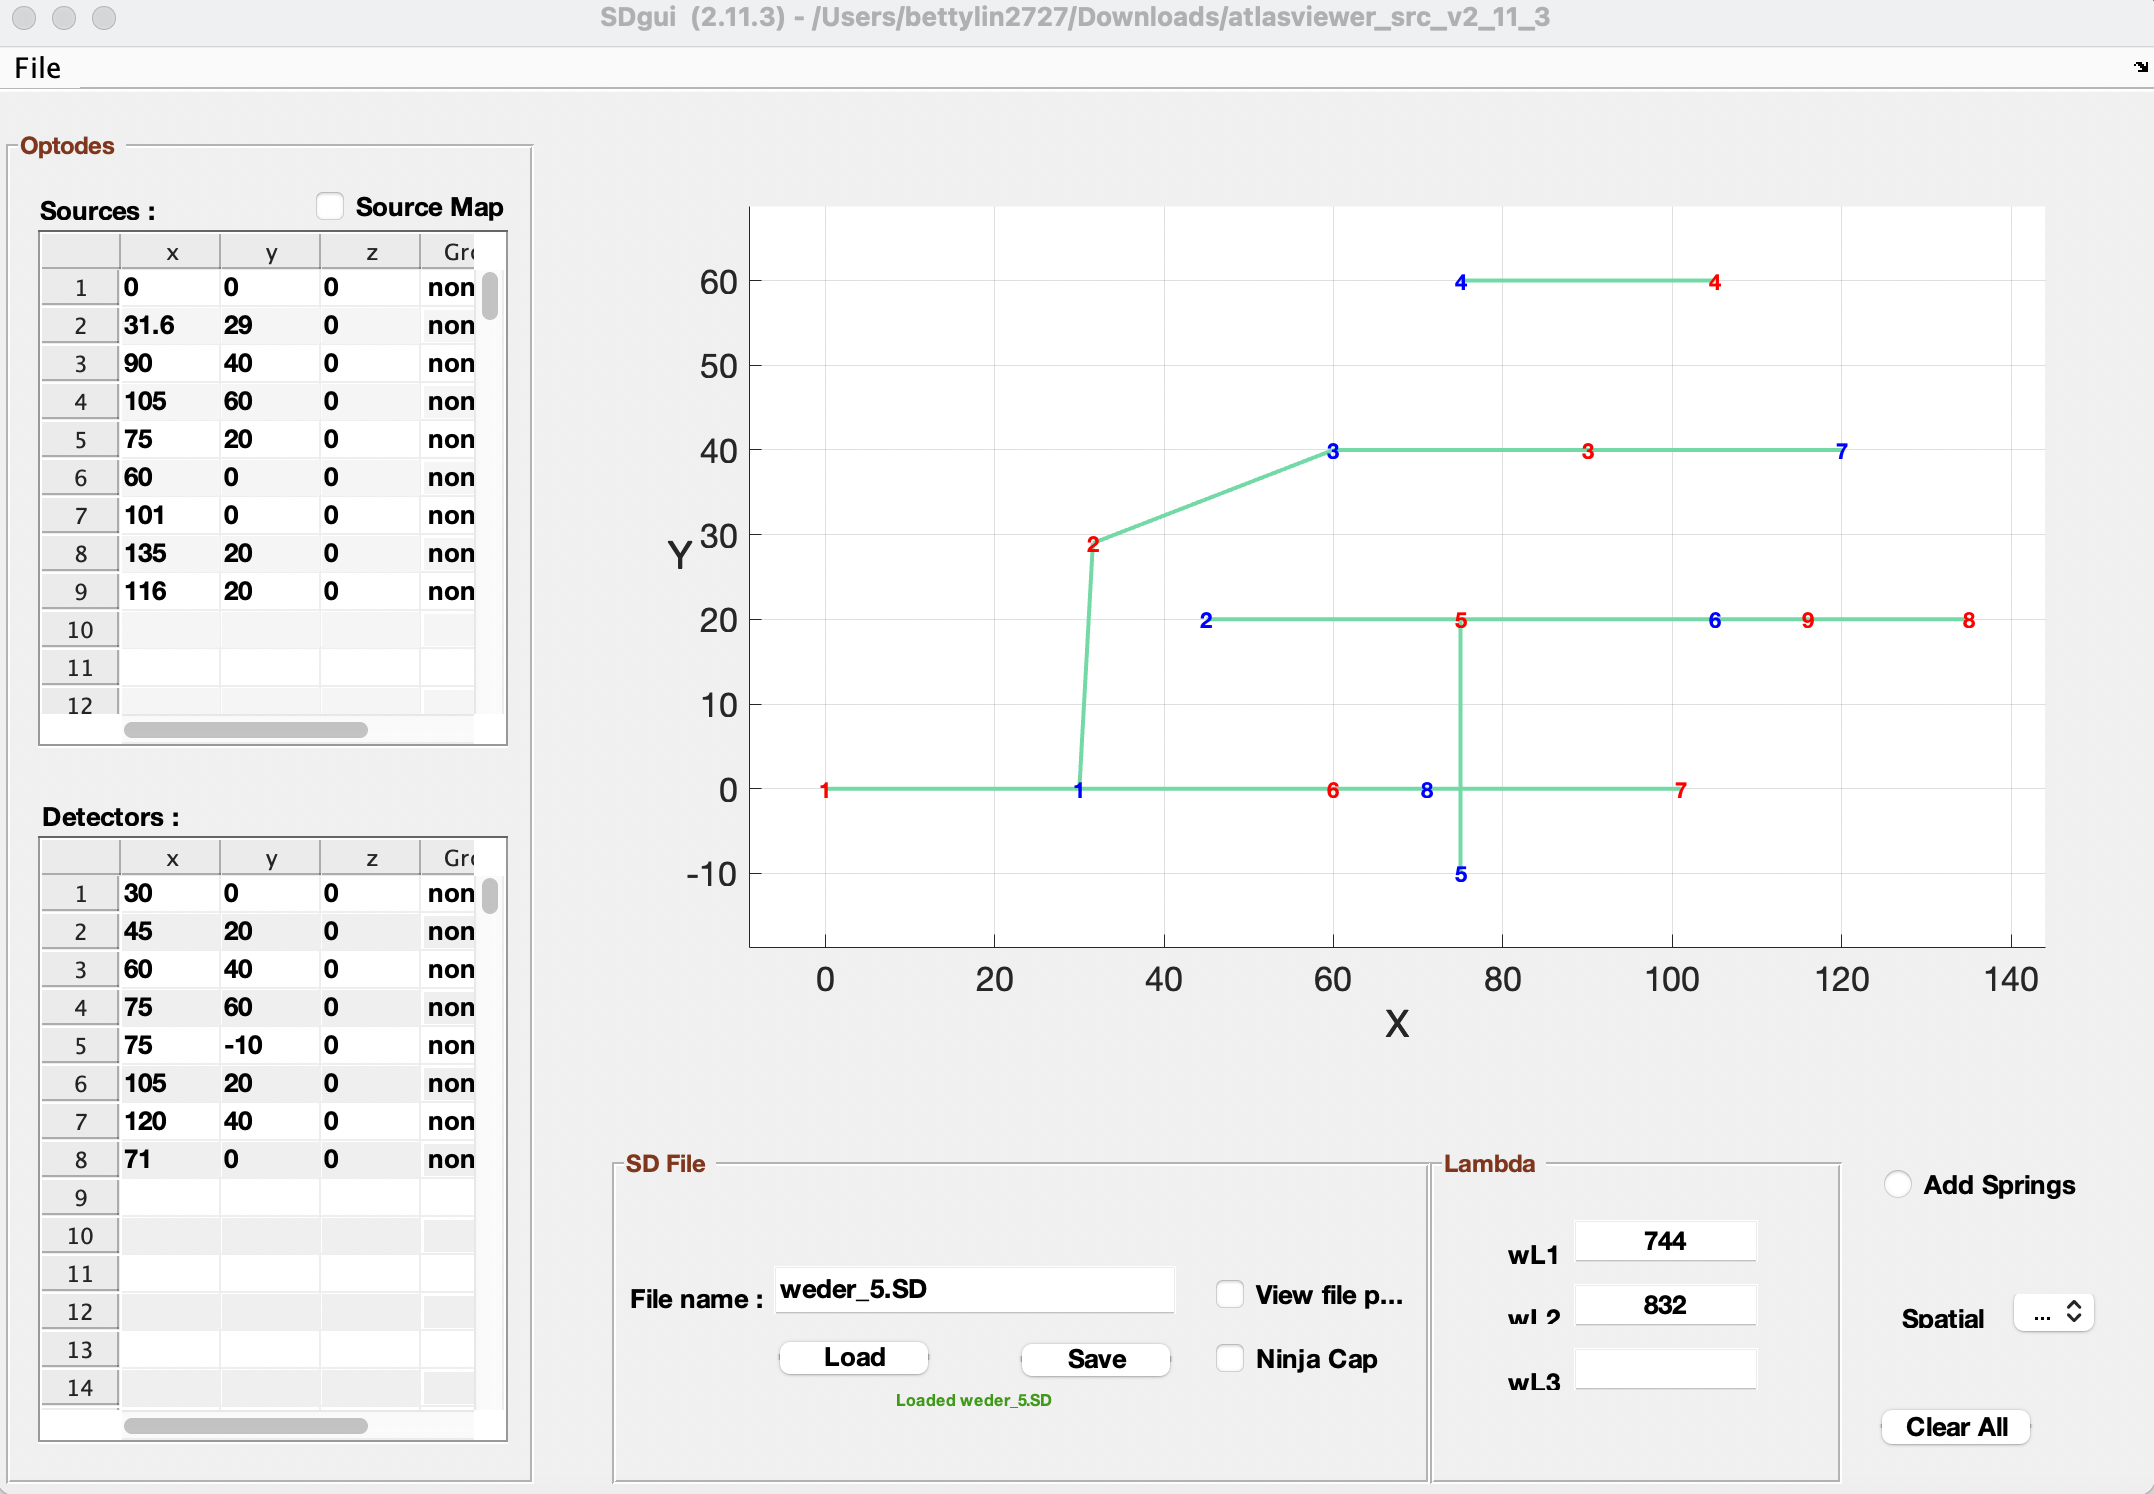
\includegraphics[scale=.35]{bilder/SDgui.png}
  \caption{SDgui interface and optode coordinates.}
  \label{fig:somesignal}
\end{figure}

\begin{figure}
\centering
\begin{minipage}[c]{.4\linewidth}
  \centering
  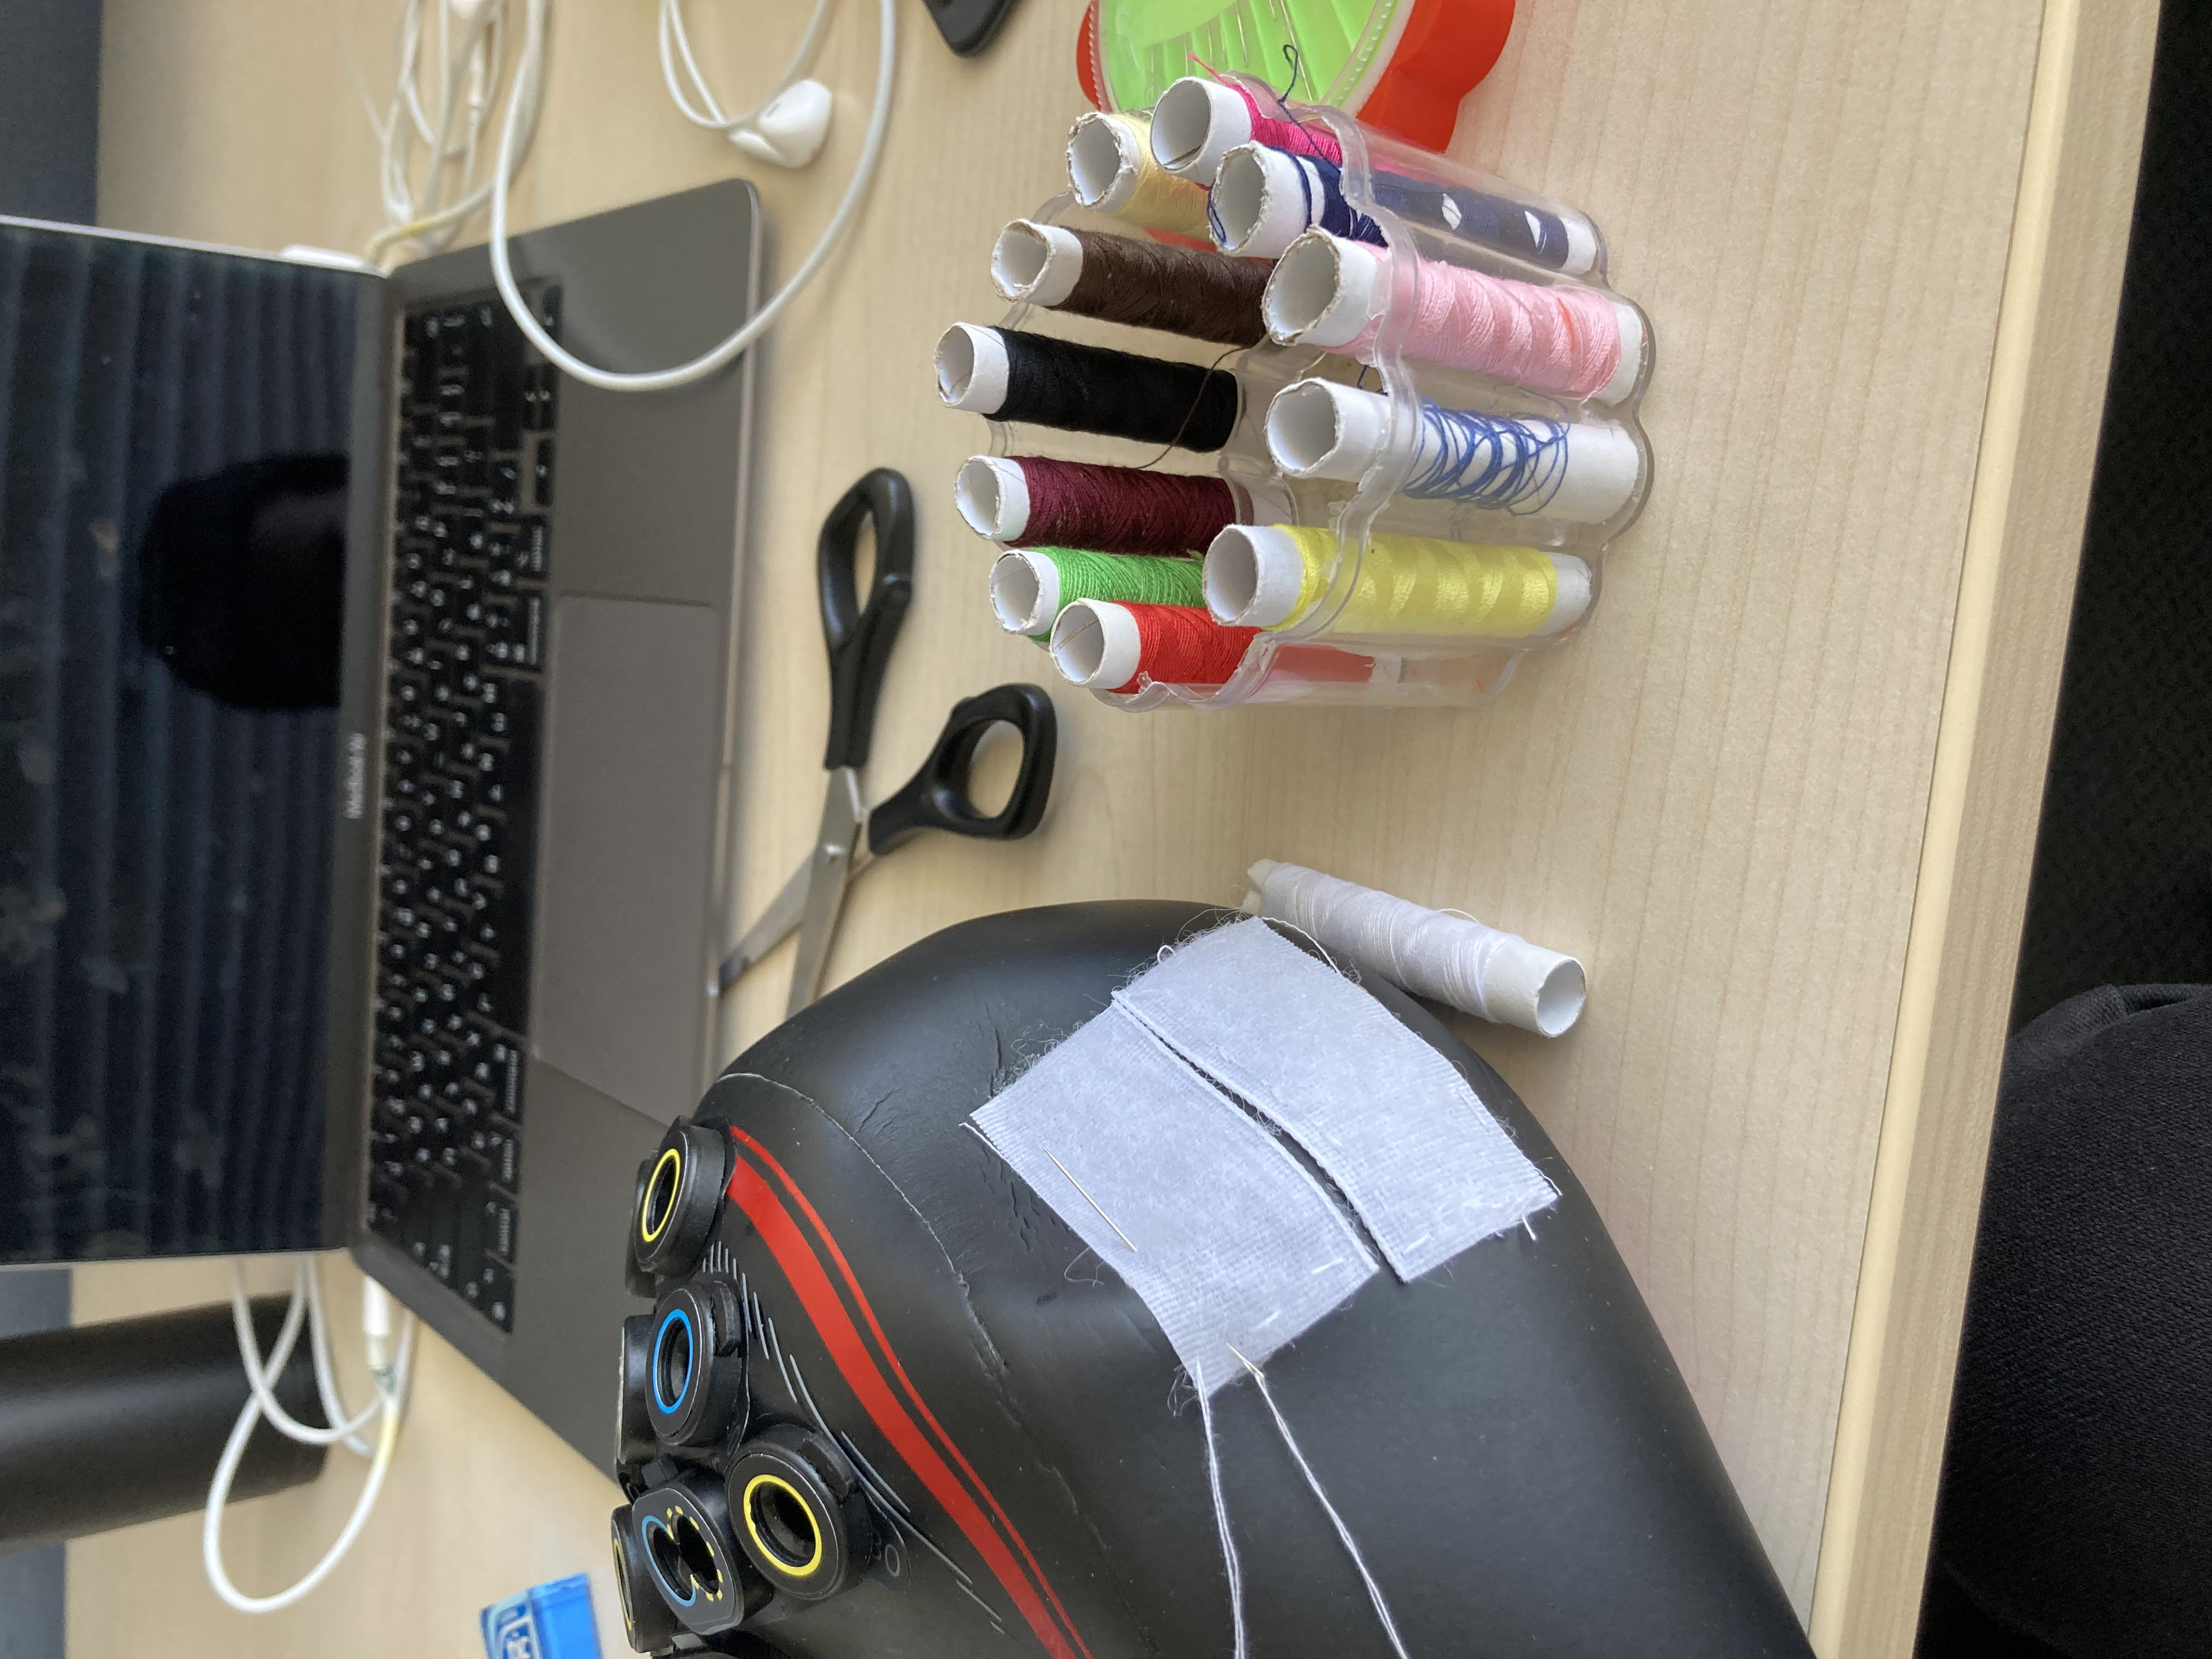
\includegraphics[scale= 0.05, angle= -90, origin= c]{bilder/IMG_9825.jpg}
  \caption{Manufacturing process of the cap}
\end{minipage} \hfill
\begin{minipage}[c]{.4\linewidth}
  \centering
  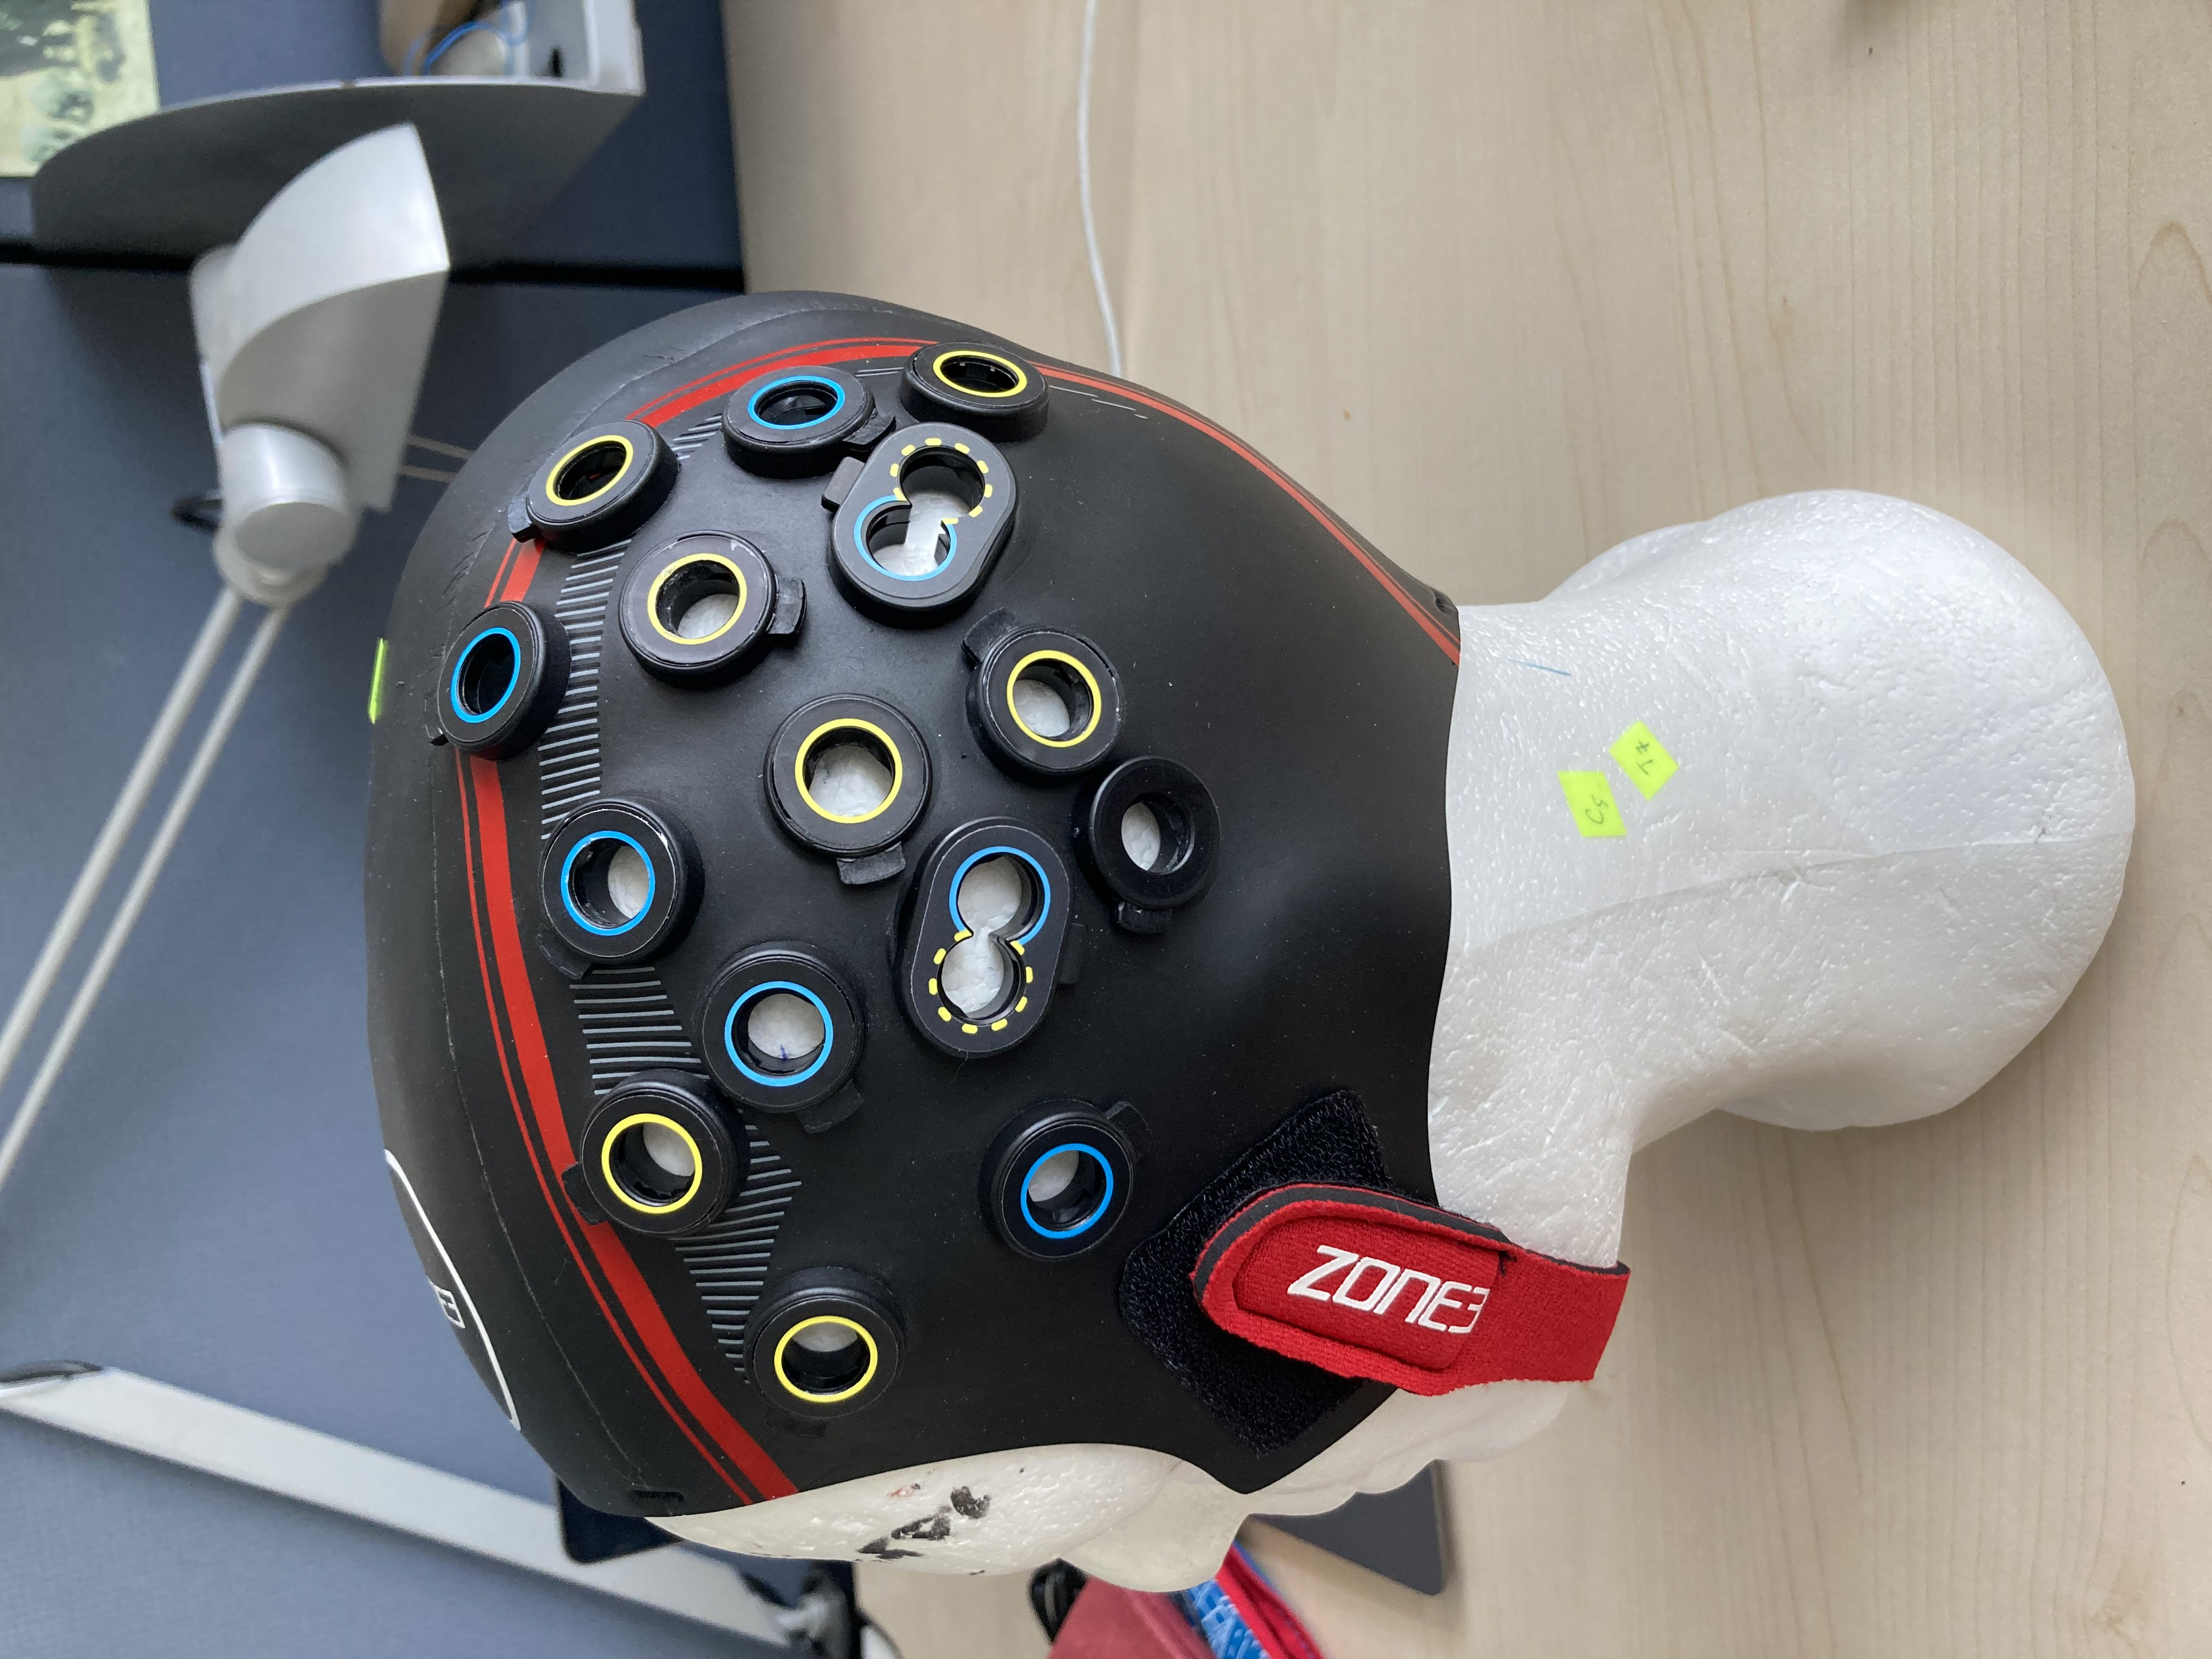
\includegraphics[scale= 0.05, angle= -90, origin= c] {bilder/IMG_9768.jpg}
  \caption{Finished cap on dummy}
  \label{fig:test2}
\end{minipage}
\end{figure}

Due to device limitations, we only measured one side of the brain. According to previous research \cite {Frost1999-vs} , language processing has been predominantly associated to cortical activity in the left hemisphere. As a result, we've decided to focus on the left hemisphere.

The fNIRS device we use also has limited number of sources and detectors. If we'd like to keep the original design, we'd need 9 sources and 9 detectors. However, the device we are using has only 10 sources and 8 detectors. Hence, we shifted one channel around T7 a little bit to the left, so that one less detector is needed. At the end, there were 12 long channels and 2 short channels in out setup.

For the software usage, an .xml file is required . In the .xml file, the sources, detectors, and channels are defined. Different optode templates for different probe design can be stored in one single .xml file. The physical cap was self-made from a swimming cap. With the help of a dummy head model, correct positions of the optodes were marked and holes were drilled accordingly. The mounts were put on the cap on the holes. In order to ensure the correct channels length to be fixed exactly at 30 mm, plastic holders were also placed on the long channels. As for the short channels, the  package comes with mounts for short channels. Thus, no plastic holders were needed in the case. The short channels were 11 mm long. The self-made cap turned out to work out well. The contacts between the scalp and the optodes were good thanks to the elastic characteristic of the material.



\section {Acoustic Stimulation during fNIRS Experiment}
Auditory stimuli were delivered binaurally via an audio metric headphone (Sennheiser HD 650). Stimuli consisted of 20-s chunks of the ICRA noise \cite {Dreschler}. 

To begin with, ICRA noise was developed to be used as background noise in clinical tests of hearing aids and possibly for measruing characteristics of non-linear instruments. The signals are based on live English speech from the EUROM database \cite {chanEUROM} in which a female speaker is explaining about the system of arithmetical notation. The speech signals were sampled with a sampling rate of 44.1 kHz. By composing the speech signals with well defined spectral and temporal characteristic, the modified signals have long-term spectrums but are completely unintelligible. 
 
We chose to use ICRA noise as stimuli based on several reasons. For one, ICRA noise is broadband amplitude-modulated signal. By selecting a broadband stimulus, broad cortical auditory areas and be activated more strongly compared with simple static stimulus. The bandwidth of auditory stimuli is positively correlated with the mean percentage signal change and spread of cortical activation \cite {Hall}. Previous fMRI study also manifested that more complex auditory stimuli elicit greater response in most parts of the auditory cortes \cite {Belin}. For the other, ICRA noise is a well-known and accessible stimulus. It is also considered as an international de facto standard for hearing research. In this way, our results can be comparable with other researches.
 
As for choosing different sound level pressure, we picked 40 dB, 65 dB, 90 dB, and silent stimulus, i.e. 0 dB. Calibrations were performed using an oscilloscope, a G.R.A.S. Power Module Type 12AK,  and an artificial ear (G.R.A.S. 43AA). The artificial ear transform the SPLs (sound pressure levels) into electrical signals, i.e. voltages that can be measured by the oscilloscope. According to the instruction manual of the G.R.A.S. artificial ear, the measured level is 11.19 $[ \frac {mV}{Pa}]$ and we know the SPL in dB is defined as 
\[
SPL [dB] = 20 \cdot log \frac{P}{P_0} \text{ , where $P_0$ is $20 \mu$Pa}
\] 
Hence, the relation between SPL and measured voltage should be.
\[
V = 20{ \mu Pa} \cdot 10^{\frac {SPL}{20}}  \cdot 10^{\frac{Gain}{20}} \cdot 11.19 {\frac {mV}{Pa}} 
\]
The headphone with the artificial ear were setup together in the sound booth to ensure minimal environmental noise. The output voltages were measured with the oscilloscope. This way, the corresponding amplitude inputs for later MATLAB scripts for the desire SPLs can be determined.

MATLAB and Oxysoft were used during the measurement. In MATLAB, a chunk in the ICRA audio files was selected. It was multiplied with different amplitude levels for 4 SPLs and ramped by a 10-ms Hanning window. In each epoch, all four stimuli (0dB, 40 dB, 65 dB, and 90 dB) were played randomly once. After each stimulus, there was a 25-sec silence rest to wait for the hemodynamic response. For each participant, 8 epochs were conducted. The stimuli were marked with Labstreaminglayer to note which SPL it was. This Labstreaminglayer also acted as an interface between MATLAB and Oxysoft, so that Oxysoft could mark the time for each stimulus in the measurement data correctly in real time.

\section {fNIRS Setup}
The Brite23 was used in this research. It is light weight, has 10 sources and 8 detectors and can support up to 23 channels. The Brite23 fNIRS device was connected via bluetooth to the PC and the Oxysoft software. For each measurement, the DPF is calculated depends on the age of the participant. The sampling rate was fixed at 50 Hz, for enough resolution but not unnecessary too large in terms of data size.

After the setting in the Oxysoft software was done, the participant would be asked to put on the self-made cap. On each optode position, the hair would be put aside gently with a Q-tip to ensure better contact between the optodes and the scalp. Then, the participants would be asked to put on the headphone and go into the sound booth.


\section {Data preprocession}
Data preprocessing and analysis was executed in MATLAB (Mathworks, USA) and the Homer3 toolbox. The following steps were executed.

First, the hemodynamic response was extracted with the Homer3 toolbox. Raw data were converted into optical densities. Motion artifacts were removed by using wavelet transformation of the data. The Homer3 toolbox bandpass filter (0.01 and 0.5 Hz) reduced drift, broadband noise, heartbeat, and respiration artifacts. Concentration if oxygenated and deoxygenated hemogloblin were estimated by applying the modified Beer-Lambert Law  \cite {Delpy_1988}. Strictly speaking, the DPF should be experimentally obtained with FD-NIRS or TD-NIRS. However, due to device limitation, it is not possible in this project. Hence, in our research, the DPF was determined by wavelengths of the fNIRS device and age of the participant. \cite {Duncan1996MeasurementOC}. With the given literature, the DPF for two wavelength is calculated with the formulas:
\[
DPF_{744} = 5.11 + 0.106 \cdot Age[yr]^{0.723}
\]

\[
DPF_{852} = 4.67 + 0.062 \cdot Age[yr]^{0.819}
\]

The paper has only given the formulas for four wavelengths. Although we used different wavelengths $\lambda = 757 [nm]$ and $\lambda = 843 [nm]$. We are convinced that the calculated DPF would be very close to the ones calculated with the above two equations.


It is important to note that the noise due to motion artifacts, drift, broadband noise, heartbeat, and respiration artifacts need to be processed before the concentration was estimated, according to the previous research \cite {Huppert:09}.

Later on, the extracerrebral component in long channels should be reduced by using measurements from the short channels as follows: the first principal components from the two short channels were estimated and then multiplied by its coefficient from the GLM (general linear model).However, this is not done in the scope of this research. The coefficient from the GLM were very small. They were of the magnitudes $10^{-16}$ , whereas the hemodynamic response in the long channels were of the magnitudes $10^{-5}$. Hence, we concluded the extracerrebral components in our case can be negligible.

Channels with unusable data were excluded here for further analysis. The scalp coupling index (SCI) is a common measure in this case. It is originally described in \cite {polloniniSCI}. In short, the SCI estimates the correlation between the two wavelength channels in the cardiac band as the following:

First, the signal is bandpass-filtered to keep only the cardiac band. In our case, a wide band of [0.5 - 2.5] Hz was chosen. Then, amplitude normalization is performed, and the SCI computation is defined as the absolute cross-correlation value at 0-time lag.


\begin{figure}[H]
  \centering
    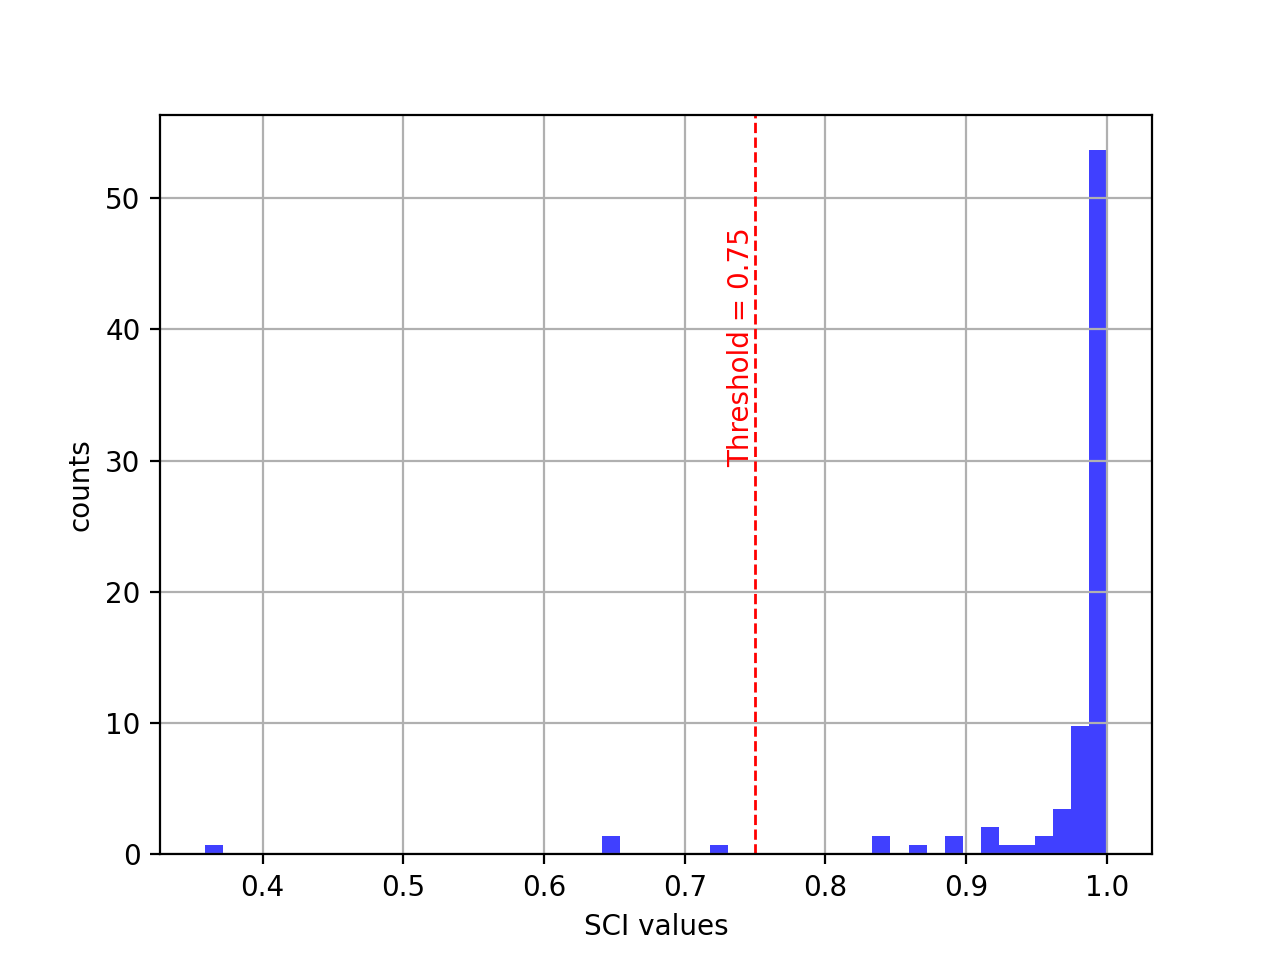
\includegraphics[scale=.75]{bilder/SCI_hist.png}
  \caption{Distribution of SCI values.}
   \label{fig:somesignal}
    \medskip
     \small {In this project, only 4 channels failed to reach the threshold = 0.75. In other words, of all the measurements (14 channels per participant, 8 participants in total.) That means over 96\% of the measurements passed the SCI threshold.}
 
\end{figure}




